\begin{center}
  \Large
  \textbf{BIOGRAFI PENULIS}
\end{center}

\addcontentsline{toc}{chapter}{BIOGRAFI PENULIS}

\vspace{2ex}

\begin{wrapfigure}{L}{0.4\textwidth}
  \centering
  \vspace{-3ex}
  % Ubah file gambar berikut dengan file foto formal Anda
  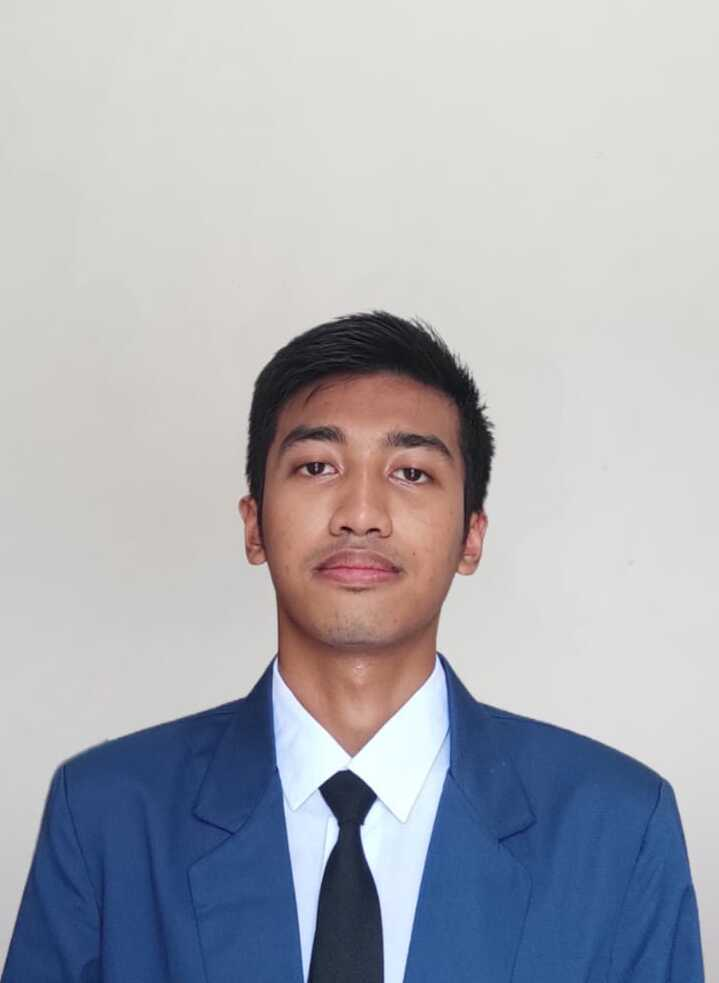
\includegraphics[width=0.4\textwidth]{gambar/foto-formal.jpeg}
  \vspace{-4ex}
\end{wrapfigure}

\name{}, biasa disapa Ikhwan, adalah mahasiswa tingkat akhir Program Studi S1 Teknik Komputer di Fakultas Teknologi Elektro dan Informatika Cerdas, Institut Teknologi Sepuluh Nopember (ITS), Surabaya. Lahir di Bogor pada 24 Desember 2003, Ikhwan menempuh pendidikan dasar di SD Nasional Plus Tunas Iblam (2009–2015), pendidikan menengah pertama di SMP Muhammadiyah MBS Al-Amin Bojonegoro (2015–2018), dan pendidikan menengah atas di SMA Al-Wafi Islamic Boarding School (2018–2021).

Selama masa perkuliahan, Ikhwan aktif berkontribusi dalam berbagai kegiatan akademik dan organisasi kampus. Ia menjabat sebagai Computer Vision Engineer di Barunastra ITS RoboBoat Team pada periode 2023–2024, berfokus pada pengembangan teknologi visi komputer untuk aplikasi robotika laut. Ia juga aktif sebagai grader di beberapa mata kuliah terkait bidang teknik komputer, membantu penilaian dan evaluasi tugas mahasiswa serta mendukung proses pembelajaran secara efektif.

Ikhwan juga memiliki pengalaman magang di PT. XL Axiata Tbk (sekarang XLSMART) dalam program X-Camp Rumah IoT Indonesia. Selama magang, ia terlibat dalam pengembangan perangkat portabel untuk deteksi alat pelindung diri menggunakan SSD MobileNetV2 yang di-deploy pada Jetson Nano, serta solusi berbasis web untuk inspeksi jalan dengan deteksi dan estimasi ukuran lubang jalan.

Di luar kegiatan akademik, Ikhwan aktif dalam pengembangan perangkat lunak dan penelitian. Ia memiliki minat khusus dalam bidang Internet of Things (IoT), visi komputer, dan pengembangan backend. Beberapa proyek yang telah dikerjakannya antara lain \emph{website} profil Lab MIoT dan inamarine-vision, aplikasi deteksi objek dan pengenalan gerakan untuk operasi \emph{crane} di Barunastra ITS yang dipamerkan di Inamarine 2024 yang dilaksanakan di Jakarta International Expo, Kemayoran.

Ikhwan memiliki keterampilan teknis dalam berbagai bahasa pemrograman dan teknologi, termasuk Python, JavaScript (Node.js, Express.js), TypeScript, OpenCV, TensorFlow, PostgreSQL, MongoDB, dan AWS. Ia juga aktif di platform GitHub dengan nama pengguna @wannn-one, tempat ia membagikan proyek-proyek open-source dan portofolio pribadinya.

Dengan visi untuk berkontribusi dalam pengembangan teknologi cerdas yang bermanfaat bagi masyarakat, Ikhwan berencana melanjutkan studi dan karier di bidang teknologi informasi, khususnya dalam solusi berbasis AI dan IoT.

Ikhwan dapat dihubungi melalui email: ikhwanulabiyu@gmail.com.